\section{Задачи на построение}

\paragraph{Предварительное замечание.}\label{1938/61}
Теоремы, доказанные нами ранее, позволяют решать некоторые задачи на \so{построение}.
Заметим, что в элементарной геометрии рассматриваются только такие построения, которые могут быть выполнены с помощью \so{линейки и циркуля}.
Употребление чертёжного треугольника и некоторых других приборов хотя и допускается ради сокращения времени, но не является необходимым.

\paragraph{}\label{1938/62}
\so{Задача 1}.
\emph{Построить треугольник по трём его сторонам $a$, $b$ и $c$} (рис.~\ref{1938/ris-65}).

\begin{figure}[!ht]
\centering
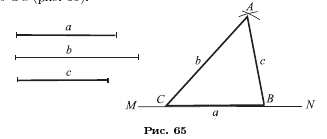
\includegraphics{mppics/ris-65}
\caption{}\label{1938/ris-65}
\end{figure}

На какой-нибудь прямой $MN$ откладываем отрезок $CB$, равный одной из данных сторон, например $a$.
Описываем две небольшие дуги с центрами в точках $C$ и $B$, одну радиусом, равным $b$, другую радиусом, равным $c$.
Точку $A$, в которой эти дуги пересекаются, соединяем с $B$ и С;
$\triangle ABC$ будет искомый.

{\small

\smallskip
\so{Замечание}.
Чтобы три отрезка могли служить сторонами треугольника, необходимо и достаточно, чтобы больший из них был меньше суммы двух остальных (необходимость доказана в §~\ref{1938/50}, условие равносильное достаточности же будет принято за очевидное утверждение в \ref{1914/118}).

}

\paragraph{}\label{1938/63}
\so{Задача 2}.
\emph{Построить угол, равный данному углу $ABC$, одной из сторон которого является данная прямая и вершина которого находится в данной точке $O$} (точка $O$ расположена на прямой $MN$, рис.~\ref{1938/ris-66}).

\begin{figure}[!ht]
\centering
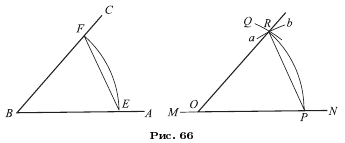
\includegraphics{mppics/ris-66}
\caption{}\label{1938/ris-66}
\end{figure}

Описываем произвольным радиусом с центром в вершине $B$ между сторонами данного угла дугу $EF$;
затем, не изменяя раствора циркуля, переносим его остриё в точку $O$ и описываем дугу $PQ$.
Далее описываем дугу $ab$ с центром в точке $P$ радиусом, равным расстоянию между точками $E$ и $F$.
Наконец, через точки $O$ и $R$ (пересечение двух дуг) проводим прямую.
Угол $ROP$ равен углу $ABC$, потому что треугольники $ROP$ и $FBE$, имеющие соответственно равные стороны, равны.

\begin{wrapfigure}{o}{40mm}
\vskip-4mm
\centering
\includegraphics{mppics/ris-67}
\caption{}\label{1938/ris-67}
\bigskip
\includegraphics{mppics/ris-68}
\caption{}\label{1938/ris-68}
\end{wrapfigure}

\paragraph{}\label{1938/64}
\mbox{\so{Задача 3}.}
\emph{Разделить данный угол $ABC$ пополам (рис.~\ref{1938/ris-67}), другими словами, построить биссектрису данного угла или провести его ось симметрии.}
С центром в вершине $B$ произвольным радиусом опишем между сторонами угла дугу $DE$.
Затем, взяв произвольный раствор циркуля, больший, однако, половины расстояния между точками $E$ и $D$ (смотри замечание к задаче 1), описываем этим раствором небольшие дуги с центрами в точках $D$ и $E$, которые пересекутся в некоторой точке $F$.
Проведя прямую $BF$, мы получим биссектрису угла $ABC$.


Для доказательства соединим прямыми точку $F$ с $D$ и $E$;
тогда получим два треугольника $BEF$ и $BDF$, которые равны, так как у них $BP$ — общая сторона\footnote{На чертежах общая сторона треугольников обычно обозначается значком похожим на $S$.}, $BD=BE$ и $DF=EF$ по построению.
Из равенства треугольников следует:
$\angle ABF = \angle CBF$.

\paragraph{}\label{1938/65}
\so{Задача 4}.
Из данной точки $C$ прямой $AB$ восстановить к этой прямой перпендикуляр (рис.~\ref{1938/ris-68}).

Отложим на $AB$ по обе стороны от данной точки $C$ равные отрезки (произвольной длины) $CD$ и $CE$.
С центрами в точках $E$ и $D$ одним и тем же раствором циркуля (б\'{о}льшим, однако, $CD$) опишем две небольшие дуги, которые пересекутся в некоторой точке $F$.
Прямая, проведённая через точки $C$ и $F$, будет искомым перпендикуляром.

Действительно, как видно из построения, точка $F$ одинаково удалена от точек $D$ и $E$;
следовательно, она должна лежать на срединном перпендикуляре к отрезку $DE$ (§~\ref{1938/58});
но середина этого отрезка есть $C$, а через точки $C$ и $F$ можно провести только одну прямую;
значит, $FC \perp DE$.

\paragraph{}\label{1938/66}
\so{Задача 5}.
\emph{Из данной точки $A$ опустить перпендикуляр на данную прямую $BC$} (рис.~\ref{1938/ris-69}).

\begin{wrapfigure}{o}{41mm}
\centering
\includegraphics{mppics/ris-69}
\caption{}\label{1938/ris-69}
\bigskip
\includegraphics{mppics/ris-70}
\caption{}\label{1938/ris-70}
\end{wrapfigure}

С центром в точке $A$ произвольным раствором циркуля (б\'{о}льшим, однако, расстояния от $A$ до $BC$) опишем дугу, которая пересечётся с $BC$ в каких-нибудь точках $D$ и $E$.
С центрами в этих точках произвольным, но одним и тем же раствором циркуля (б\'{о}льшим, однако, $\tfrac12\cdot DE$), проводим две небольшие дуги, которые пересекутся между собой в некоторой точке $F$.
Прямая $AF$ будет искомым перпендикуляром.

Действительно, как видно из построения, каждая из точек $A$ и $F$ одинаково удалена от $D$ и $E$, а такие точки лежат на срединном перпендикуляре к отрезку $DE$ (§~\ref{1938/58}).

\paragraph{}\label{1938/67}
\mbox{\so{Задача 6}.}
\emph{Провести срединный перпендикуляр к данному отрезку \emph{($AB$)}} (рис.~\ref{1938/ris-70}).

Произвольным, но одинаковым раствором циркуля (б\'{о}льшим $\tfrac12\cdot AB$) описываем две дуги с центрами в точках $A$ и $B$, которые пересекутся между собой в некоторых точках $C$ и $D$.
Прямая $CD$ будет искомым перпендикуляром.
Действительно, как видно из построения, каждая из точек $C$ и $D$ одинаково удалена от $A$ и $B$;
следовательно, эти точки должны лежать на оси симметрии отрезка $AB$.

\smallskip
\so{Задача 7}.
\emph{Разделить пополам данный отрезок} (рис.~\ref{1938/ris-70}).
Решается так же, как предыдущая задача.

\paragraph{Пример более сложной задачи.}\label{1938/68}
При помощи этих основных задач можно решать задачи более сложные.
Для примера решим следующую задачу.

\smallskip
\so{Задача}.
\emph{Построить треугольник, зная его основание $B$, угол $\alpha$, прилежащий к основанию, и сумму $s$ двух боковых сторон} (рис.~71).

\begin{figure}[!ht]
\centering
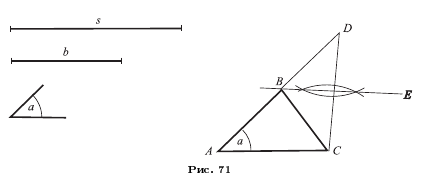
\includegraphics{mppics/ris-71}
\caption{}\label{1938/ris-71}
\end{figure}

Чтобы составить план решения, предположим, что задача решена, то есть что найден такой $\triangle ABC'$, у которого основание $AC = b$, $\angle A=\alpha$ и $AB+BC=s$.
Рассмотрим полученный чертёж.
Сторону $AC$, равную $b$, и угол $A$, равный $\alpha$, мы построить умеем.
Значит, остаётся найти на другой стороне угла $A$ такую точку $B$, чтобы сумма $AB+BC$ равнялась $s$.
Продолжив $AB$, отложим отрезок $AD$, равный $s$.

Вопрос сводится к тому, чтобы на прямой $AB$ отыскать такую точку $B$, которая была бы одинаково удалена от $C$ и $D$.
Такая точка, как мы знаем (§~\ref{1938/58}), должна лежать на срединном перпендикуляре к отрезку $CD$. 
Точка $B$ найдётся в пересечении этого срединного перпендикуляра с $AD$. 

Итак, вот решение задачи:
строим (рис.~\ref{1938/ris-71}) угол $A$, равный данному углу $\alpha$;
на сторонах его откладываем $AC=b$ и $AD=s$ и соединяем точку $D$ с $C$.
Проведём срединный перпендикуляр к отрезку $CD$;
пересечение его с $AD$, то есть точку $B$, соединяем с $C$.
Треугольник $ABC$ будет  искомый, так как он удовлетворяет всем требованиям задачи:
у него $AC=b$, $\angle A = \alpha$ и $AB+BC=s$ (потому что $BD=BC$).

Рассматривая построение, мы замечаем, что решения задачи может не быть.
Действительно, если сумма задана слишком малой сравнительно с $b$, то перпендикуляр $BE$ может не пересечь отрезка $AD$ (или пересечёт его продолжение за точку $A$ или за точку $D$);
в этом случае задача не имеет решения.
И независимо от построения можно видеть, что решения нет, если $s<b$ или $s=b$, потому что не может быть такого треугольника, у которого сумма двух сторон была бы меньше или равна третьей стороне.

Если задача имеет решение, то оно единственно;
то есть существует только один треугольник, удовлетворяющий требованиям задачи, так как перпендикуляр $BE$ может пересечься с прямой $AD$ только в одной точке.

{\small

\paragraph{}\label{1938/69}
\so{Замечание}.
Из приведённого примера видно, что решение сложной задачи на построение состоит из следующих четырёх частей.

1) Предположив, что задача решена, делают от руки приблизительный чертёж;
искомой фигуры и затем, внимательно рассматривая начерченную фигуру, стремятся найти такие зависимости между данными задачи и искомыми, которые позволили бы свести задачу к другим, известным ранее.
Эта самая важная часть решения задачи, имеющая целью составить план решения, носит название \textbf{анализа}.

2) Когда таким образом план решения найден, выполняют сообразно ему \textbf{построение}.

3) Для проверки правильности плана показывают затем на основании известных теорем, что полученная фигура удовлетворяет всем требованиям задачи.
Эта часть называется \textbf{синтезом}.

4) Затем задаются вопросом, при всяких ли данных задача имеет решение, допускает ли она одно решение или несколько, и нет ли в задаче каких-либо особенных случаев, когда построение упрощается или, наоборот, усложняется.
Эта часть решения называется \textbf{исследованием} задачи.

Когда задача очень проста и не может быть сомнения относительно существования её решения, то обыкновенно анализ и исследование опускают, а указывают прямо построение и приводят доказательство.
Так мы делали, излагая решение первых семи задач этой главы;
так же будем делать и впоследствии, когда нам придётся излагать решения несложных задач.

}

{\small

\subsection*{Упражнения}

\begin{center}\so{Доказать теоремы}
\end{center}

\begin{enumerate}[noitemsep]

\item
В равнобедренном треугольнике две медианы равны, две биссектрисы равны, две высоты равны.

\item
Если к каждой из равных сторон равнобедренного треугольника восстановим срединные перпендикуляры до пересечения с другой из равных сторон, то эти перпендикуляры будут равны. 

\item
Прямая, перпендикулярная к биссектрисе угла, отсекает от его сторон равные отрезки.

\item
Медиана треугольника меньше его полупериметра.

\item
Медиана треугольника меньше полусуммы сторон, между которыми она заключается.

\smallskip
\so{Указание}.
Продолжить медиану на расстояние, равное ей, полученную точку соединить с одним концом стороны, к которой проведена медиана, и рассмотреть образовавшуюся фигуру.

\item
Сумма медиан треугольника меньше периметра, но больше полупериметра.

\smallskip
\so{Указание}.
См. предыдущее упражнение, а также следствие в §~\ref{1938/50}.

\item
Сумма диагоналей четырёхугольника меньше его периметра, но больше полупериметра.

\item
Доказать как прямую теорему, что всякая точка, не лежащая на срединном перпендикуляре к отрезку, неодинаково удалена от концов этого отрезка, а именно: 
она ближе к тому концу, с которым она расположена по одну сторону от перпендикуляра.

\item
Доказать как прямую теорему, что всякая точка, не лежащая на биссектрисе угла, неодинаково отстоит от сторон его.

\item %%%%overfull
Медиана, исходящая из какой-нибудь вершины треугольника, равно отстоит от двух других его вершин.

\item
На одной стороне угла $A$ отложены отрезки $AB$ и $AC$ и на другой стороне отложены отрезки $AB'=AB$ и $AC' = AC$.
Доказать, что прямые $BC'$ и $B'C$ пересекаются на биссектрисе угла $A$.

\item
Вывести отсюда способ построения биссектрисы угла.

\item
Если $A'$ и $A$, $B'$ и $B$ — две пары точек, симметричных относительно какой-нибудь прямой $XY$, то четыре точки $A'$, $A$, $B'$, $B$ лежат на одной окружности.

\item
Дан острый угол $XOY$ и точка $A$ внутри этого угла.
Найти на стороне $OX$ точку $B$ и на стороне $OY$ точку $C$ так, чтобы периметр $\triangle ABC$ был наименьший.

\smallskip
\so{Указание}.
Надо взять точки, симметричные с $A$ относительно сторон $OX$ и $OY$.

\end{enumerate}

\begin{center}
\so{Задачи на построение}
\end{center}

\begin{enumerate}[resume,noitemsep]

\item
Построить сумму двух, трёх и более углов.

\item
Построить разность двух углов.

\item
По данной сумме и разности двух углов найти эти углы.

\item
Разделить угол на 4, 8 и 16 равных частей.

\item
Через вершину данного угла провести вне его такую прямую, которая со сторонами угла образовала бы равные углы.

\item
Построить треугольник:
а) по двум сторонам и углу между ними;
б) по стороне и двум прилежащим углам;
в) по двум сторонам и углу, лежащему против б\'{о}льшей из них;
г) по двум сторонам и углу, лежащему против меньшей из них (в этом случае получаются два решения, или одно, или ни одного).

\item
Построить равнобедренный треугольник:
а) по основанию и боковой стороне;
б) по основанию и прилежащему углу;
в) по боковой стороне и углу при вершине;
г) по боковой стороне и углу при основании.

\item
Построить прямоугольный треугольник:
а) по двум катетам;
б) по катету и гипотенузе;
в) по катету и прилежащему острому углу.

\item
Построить равнобедренный треугольник:
а) по высоте и боковой стороне;
б) по высоте и углу при вершине;
в) по основанию и перпендикуляру, опущенному из конца основания на боковую сторону.

\item
Построить прямоугольный треугольник по гипотенузе и острому углу.

\item
Через точку, данную внутри угла, провести такую прямую, которая отсекла бы от сторон угла равные части.

\item
По данной сумме и разности двух отрезков найти эти отрезки.

\item
Разделить данный отрезок на 4, 8, 16 равных частей.

\item
На данной прямой найти точку, одинаково удалённую от двух данных точек (вне прямой).

\item
Найти точку, равно отстоящую от трёх вершин треугольника.

\item
На прямой, пересекающей стороны угла, найти точку, одинаково удалённую от сторон этого угла.

\item
Найти точку, одинаково удалённую от трёх сторон треугольника.

\item
На бесконечной прямой $AB$ найти такую точку $C$, чтобы полупрямые $CM$ и $CN$, проведённые из $C$ через данные точки $M$ и $N$, расположенные по одну сторону от $AB$, составляли с полупрямыми $CA$ и $CD$ равные углы.

\smallskip
\so{Указание}.
Построить точку $M'$, симметричную с $M$ относительно оси $AB$, и соединить $M'$ с $N$.

\item
Построить прямоугольный треугольник по катету и сумме гипотенузы с другим катетом.

\item
Построить треугольник по основанию, углу, прилежащему к основанию, и разности двух других сторон.
(Рассмотреть два случая:
1) когда дан меньший из двух углов, прилежащих к основанию;
2) когда дан больший из них.)

\smallskip
\so{Указание}.
См. задачу §~\ref{1938/68}.

\item
Построить прямоугольный треугольник по катету и разности двух других сторон.

\item
Дан угол $A$ и точки $B$ и $C$, расположенные одна на одной стороне угла, другая — на другой.
Найти:
1) точку $M$, равно отстоящую от сторон угла, и такую, чтобы $MC=MB$;
2) точку $N$, равно отстоящую от сторон угла так, чтобы $NC=CB$.

\item
По соседству с железной дорогой расположены две деревни $A$ и $B$.
Найти на линии железной дороги (имеющей прямолинейную форму) место для станции, которая была бы одинаково удалена от $A$ и $B$.

\item
Дан угол $A$ и точка $B$ на одной из его сторон.
Найти на другой стороне такую точку $C$, чтобы сумма $CA+CD$ была равна данному отрезку~$\ell$.

\end{enumerate}

}
